\chapter{Технологический раздел}
Цель технологического раздела – описание инструментов, средств разработки, языков программирования и технологий, использованных при реализации программного комплекса системы.
\section{Выбор и обоснование языка программирования}
В качестве языка разработка был выбран C++. Причины, по которым был выбран именно он следующие:
\begin{itemize}
	\item Статическая типизация
	\item Высокая скорость выполнения
	\item Поддержка ООП
	\item Поддержка механизма исключений
	\item Последние стандарты расширили возможности языка, за счет чего разработка становится очень удобной
\end{itemize}

Выбор среды разработка пал на Qt Creator по следующим причинам:
\begin{itemize}
	\item Удобный редактор
	\item Удобные средства отладки
	\item Поддержка псевдо-асинхронной модели программирования
	\item Большое количество встроенных библиотек
	\item Частичная платформонезависимость
\end{itemize}

\section{Интерфейс пользователя}
\begin{figure}[H]
	\centering
	{
		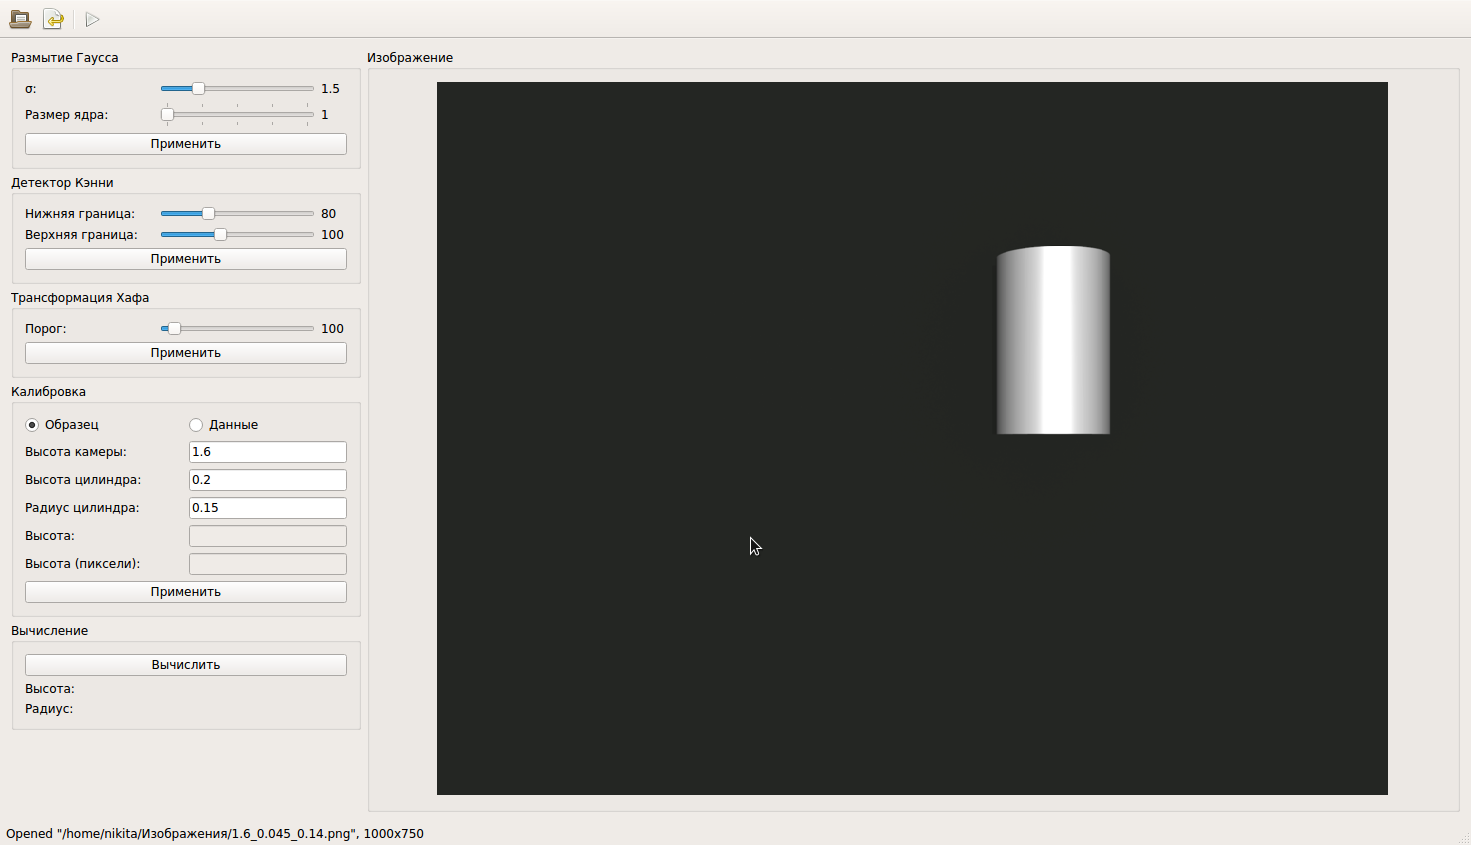
\includegraphics[scale=0.28,valign=t]{img/screen1.png}
		\caption{Главное окно.}
		\label{struct:mainwindow}}
\end{figure}
\begin{figure}[H]
	\centering
	{
		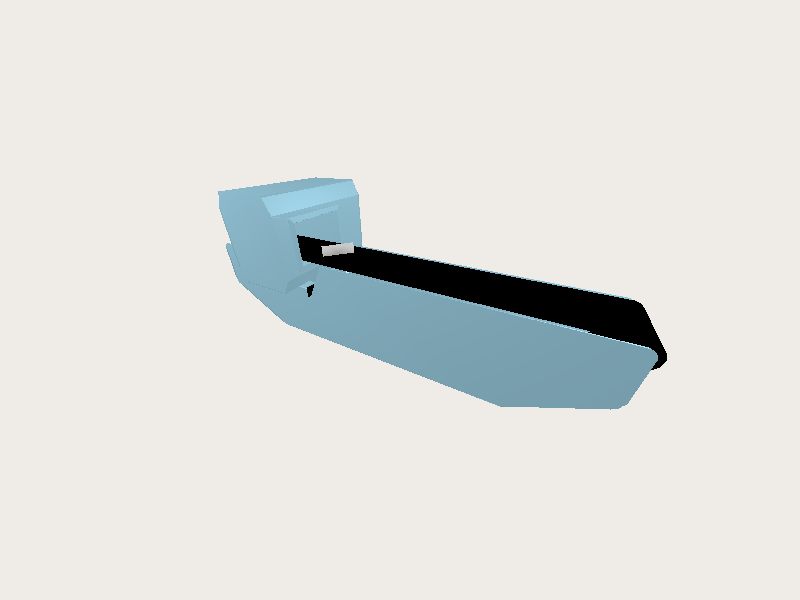
\includegraphics[scale=0.28,valign=t]{img/screen2.png}
		\caption{Окно анимации.}
		\label{struct:animation}}
\end{figure}

\section{Входные данные}
Для работы алгоритма Кэнни необходимо задать: \(\sigma \in [0..5]\) и размер ядра \(\in \overline{1,3..9}\) для сглаживания Гаусса, нижнюю и верхнюю границу пороговой фильтрации \(\in \overline{10,240}\).

Для настройки преобразования Хафа необходимо задать минимальную длину искомого отрезка \(\in \overline{10,1000}\).

Также необходимо провести калибровку системы. Сделать это можно двумя путями:
\begin{enumerate}
	\item На основе фотографии цилиндра, с известными размерами. В этом случае необходимо задать высоту камеры относительно ленты конвейера, геометрические размеры цилиндра, изображенного на фотографии.
	\item На произвольного отрезка на самой ленте конвейера. Требуется указать действительную длину этого отрезка, и длину этого отрезка на изображении в пикселях.
\end{enumerate}

\section{Основные диаграммы классов модуля нахождения размеров}
Диаграммы классов и пояснения к ним представлены на рисунках.

\begin{figure}[H]
	\centering
	\begin{minipage}{.5\textwidth}
		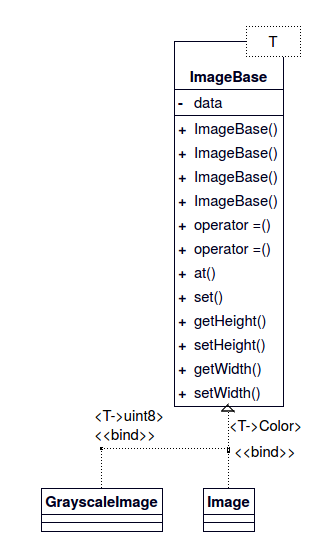
\includegraphics[scale=0.65]{classes/image.png}
		\caption{Диаграмма классов изображения.}
		\label{class:image}
	\end{minipage}%
	\begin{minipage}{.5\textwidth}
		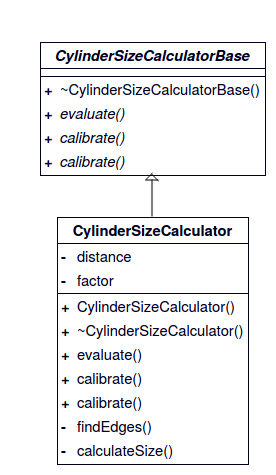
\includegraphics[scale=0.65]{classes/cylindersize.png}
		\caption{Диаграмма классов вычислительного модуля. Использован паттерн стратегия, для возможности безболезненной замены.}
		\label{class:cylindersize}
	\end{minipage}
	
\end{figure}

\begin{figure}[H]
	\centering
	\begin{minipage}{.33\textwidth}
		\centering
		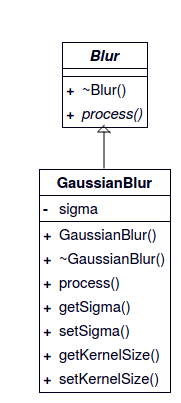
\includegraphics[scale=0.65]{classes/blur.png}
		\caption{Диаграмма классов размытия. Паттерн стратегия.}
		\label{class:blur}
	\end{minipage}%
	\begin{minipage}{.33\textwidth}
		\centering
		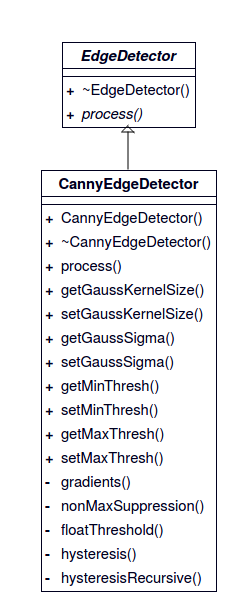
\includegraphics[scale=0.65]{classes/edgedetector.png}
		\caption{Диаграмма классов детектора границ. Паттерн стратегия.}
		\label{class:edgedetector}
	\end{minipage}
	\begin{minipage}{.33\textwidth}
		\centering
		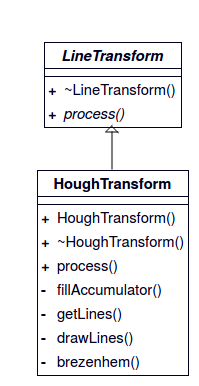
\includegraphics[scale=0.65]{classes/linetransform.png}
		\caption{Диаграмма классов детектора прямой. Паттерн стратегия.}
		\label{class:linetransform}
	\end{minipage}
\end{figure}

\section{Основные диаграммы классов модуля моделирования}
Диаграммы классов и пояснения к ним представлены на рисунках.
\begin{figure}[H]
	\centering
	\begin{minipage}{1\textwidth}
		\centering
		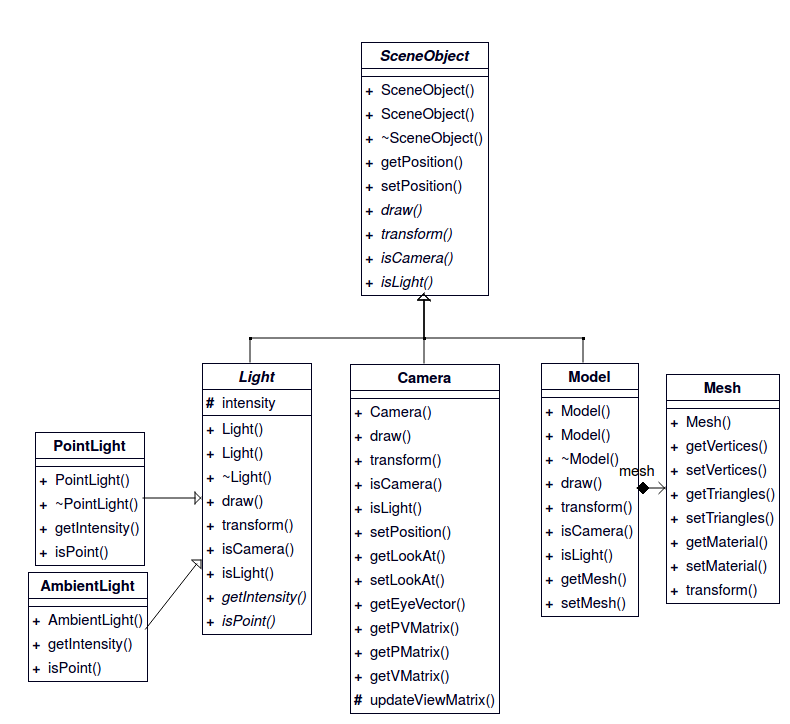
\includegraphics[scale=0.65]{classes/sceneobject.png}
		\caption{Диаграмма класс объектов сцены.}
		\label{class:sceneobject}
	\end{minipage}%
\end{figure}

\begin{figure}[H]
	\centering
	\begin{minipage}{1\textwidth}
		\centering
		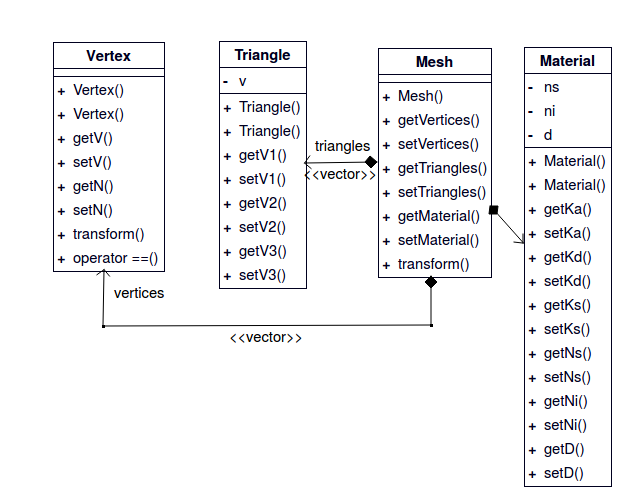
\includegraphics[scale=0.65]{classes/mesh.png}
		\caption{Диаграмма класс объектов меша.}
		\label{class:mesh}
	\end{minipage}%
\end{figure}

\begin{figure}[H]
	\centering
	\begin{minipage}{1\textwidth}
		\centering
		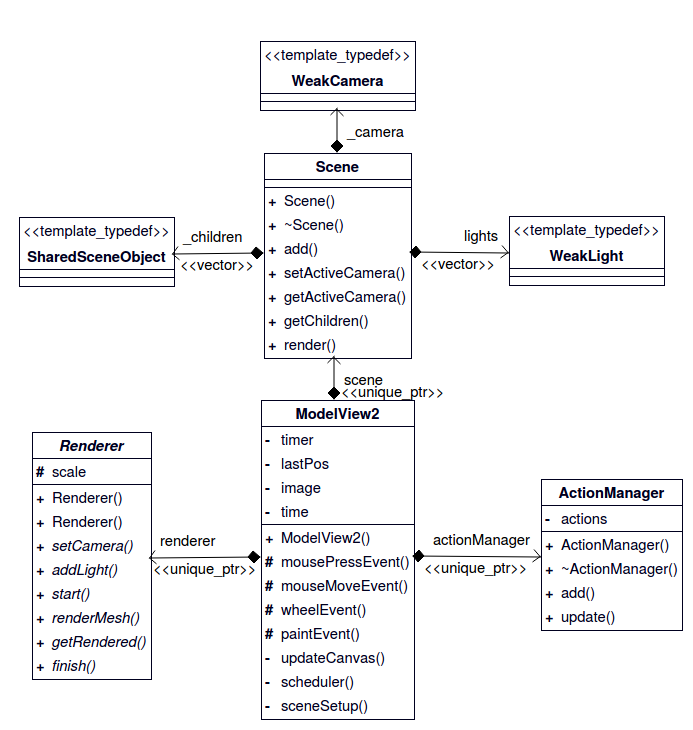
\includegraphics[scale=0.65]{classes/scene.png}
		\caption{Диаграмма классов сцены, рендера и менеджера анимаций. Для рендера использован паттерн посетитель, для абстрагирования от конкретных операций отрисовки для каждого объекта. }
		\label{class:scene}
	\end{minipage}%
\end{figure}

\begin{figure}[H]
	\centering
	\begin{minipage}{1\textwidth}
		\centering
		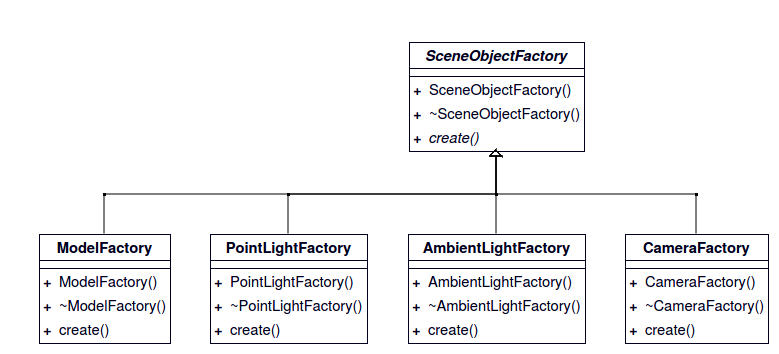
\includegraphics[scale=0.65]{classes/factory.png}
		\caption{Фабрика объектов. Паттерн фабричный метод.}
		\label{class:factory}
	\end{minipage}%
\end{figure}

\begin{figure}[H]
	\begin{minipage}{1\textwidth}
		\centering
		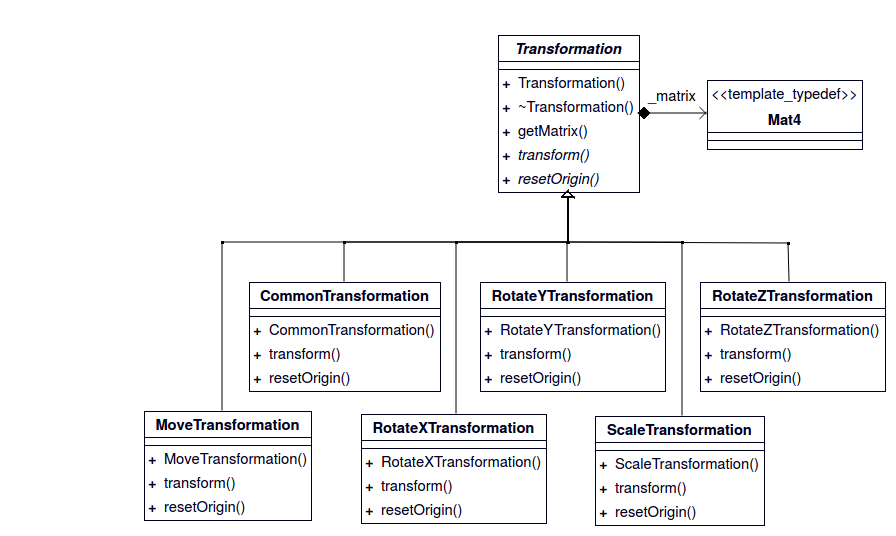
\includegraphics[scale=0.65]{classes/transformation.png}
		\caption{Диаграмма классов трансформации объектов сцены. Паттерн стратегия.}
		\label{class:transformation}
	\end{minipage}%
\end{figure}